\documentclass[12pt,a4paper]{article}

% Encodage et langue
\usepackage[T1]{fontenc}
\usepackage[utf8]{inputenc}
\usepackage[french]{babel}

% Mise en page
\usepackage[margin=2.5cm]{geometry}
\usepackage{graphicx}
\usepackage{xcolor}
\usepackage{enumitem}
\usepackage{fancyhdr}
\usepackage{titlesec}
\usepackage{booktabs}
\usepackage{array}
\usepackage{longtable}
\usepackage[colorlinks=true,linkcolor=black,citecolor=black,filecolor=black,urlcolor=black]{hyperref}
\usepackage{tikz}
\usepackage{fontawesome5}
\usepackage{float}
\usepackage{caption}

% Couleurs personnalisées (identiques aux autres guides)
\definecolor{lagoon}{RGB}{0, 128, 128}
\definecolor{sea-ink}{RGB}{0, 45, 64}
\definecolor{palm}{RGB}{46, 139, 87}
\definecolor{warn}{RGB}{230, 126, 34}
\definecolor{danger}{RGB}{231, 76, 60}
\definecolor{success}{RGB}{39, 174, 96}
\definecolor{muted}{RGB}{127, 140, 141}

% Titres
\titleformat{\section}
  {\normalfont\Large\bfseries\color{sea-ink}}{\thesection}{1em}{}
\titleformat{\subsection}
  {\normalfont\large\bfseries\color{lagoon}}{\thesubsection}{1em}{}
\titleformat{\subsubsection}
  {\normalfont\normalsize\bfseries\color{palm}}{\thesubsubsection}{1em}{}

% En-têtes et pieds de page
\setlength{\headheight}{15pt}
\pagestyle{fancy}
\fancyhf{}
\fancyhead[L]{\textcolor{sea-ink}{GLOBAL SIM GROUP — Guide Espace client}}
\fancyhead[R]{\textcolor{muted}{\leftmark}}
\fancyfoot[C]{\thepage}
\renewcommand{\headrulewidth}{0.4pt}
\renewcommand{\footrulewidth}{0pt}

% Commandes pratiques (identiques aux autres guides)
\newcommand{\screenshot}[2]{%
  \begin{figure}[H]
    \centering
    \includegraphics[width=0.95\textwidth]{#1}
    \caption{#2}
  \end{figure}%
}

\newcommand{\etape}[1]{\textbf{\faHandPointRight\ #1}}
\newcommand{\attention}[1]{\par\noindent\textcolor{warn}{\faExclamationTriangle\ Attention : #1}\par}
\newcommand{\astuce}[1]{\par\noindent\textcolor{success}{\faLightbulb\ Astuce : #1}\par}
\newcommand{\info}[1]{\par\noindent\textcolor{lagoon}{\faInfoCircle\ Info : #1}\par}

\newlist{etapes}{enumerate}{1}
\setlist[etapes]{label=\textcolor{lagoon}{\faArrowRight\ \arabic*.}, leftmargin=1.5cm, itemsep=0.4em}

\begin{document}

% Page de garde
\begin{titlepage}
  \noindent\colorbox{sea-ink}{%
    \parbox{\dimexpr\textwidth-2\fboxsep}{%
      \centering
      \vspace{1.5cm}
      
\includegraphics[height=3cm]{../logo-gsg.png}\par
      \vspace{0.6cm}
      {\Huge\bfseries\color{white} GLOBAL SIM GROUP\par}
      \vspace{0.5cm}
      {\LARGE\color{white} Guide d'utilisation — Espace client\par}
      \vspace{1.5cm}
    }%
  }

  \vfill
  \begin{center}
    {\Large\color{sea-ink} Tous les services GLOBAL SIM GROUP, depuis votre navigateur\par}
    \vspace{0.4cm}

    \begin{tikzpicture}
      \node[fill=lagoon, text=white, rounded corners=10pt, minimum width=12cm, minimum height=1.5cm, font=\large\bfseries] {Restaurant · Boutique · Pressing · Salle de fête · Séjours};
    \end{tikzpicture}
  \end{center}

  \vfill
  \begin{center}
    \textcolor{muted}{Version 1.0}
  \end{center}
\end{titlepage}

\newpage
% Table des matières
\tableofcontents
\newpage

% Introduction
\section{Avant de commencer}

L'\textbf{espace client} est votre compte en ligne chez GLOBAL SIM GROUP. Il est ouvert à toute personne disposant d'un compte client — vous n'avez pas besoin d'être résident de la résidence pour l'utiliser.

Depuis votre espace, vous pouvez :

\begin{itemize}[label=\textcolor{lagoon}{\faFile}]
  \item \textbf{Commander au restaurant} : parcourez la carte, composez votre commande (sur place, à emporter ou en livraison) et suivez sa préparation.
  \item \textbf{Faire vos achats à la boutique} : remplissez votre panier de produits et envoyez la demande — vous retirez et réglez au comptoir.
  \item \textbf{Suivre vos dépôts pressing} : l'avancement de vos linges étape par étape, avec le montant et le reste à payer.
  \item \textbf{Demander un séjour court} : une nuitée ou une sieste dans un logement de la résidence.
  \item \textbf{Réserver la salle de fête} pour vos événements.
  \item \textbf{Suivre vos abonnements} : soldes de quotas prépayés, dates de validité.
  \item \textbf{Signaler un problème} rencontré dans nos services, photos à l'appui.
\end{itemize}

\info{L'espace client est \textbf{un espace de demande et de suivi} : vous envoyez la demande en ligne, le personnel la valide (disponibilité, tarif), et le règlement se fait \textbf{sur place} (réception, comptoir, caisse). Aucun paiement ne se fait dans l'espace lui-même.}

\info{Ce que vous voyez dépend de vos \textbf{permissions}. Si un bouton « Commander » ou « Demander » n'apparaît pas, c'est que votre compte n'a pas le droit correspondant — demandez à la réception de l'ajouter. Voir le récapitulatif à la fin du guide.}

\attention{Votre espace client est \textbf{distinct du portail résident} : il ne montre ni échéances de loyer, ni caution, ni états des lieux. Ces pages appartiennent au contrat de résidence, réservé aux comptes résidents.}

\newpage

% Section 1 : Se connecter
\section{Se connecter et ouvrir votre espace}\label{sec:connexion}

Vos identifiants vous sont remis par la réception quand votre compte client est créé.

\begin{etapes}
  \item Ouvrez l'adresse de l'application dans votre navigateur.
  \item Tapez votre \textbf{identifiant} et votre \textbf{mot de passe}, puis cliquez sur \textbf{Se connecter}.
\end{etapes}

\screenshot{screenshots/espace-client/01-connexion.png}{La page de connexion}

Vous arrivez sur \textbf{« Accueil »} — la page d'accueil de votre espace client :

\screenshot{screenshots/espace-client/02-accueil.png}{L'accueil de l'espace client — vos services et le suivi en direct}

En haut de page, la \textbf{barre de navigation} donne accès à tout : Accueil, Restaurant, Boutique, Pressing, Salle de fête, Résidence, Abonnements, Mes demandes. À droite vous trouvez :

\begin{itemize}[label=\textcolor{lagoon}{\faArrowRight}]
  \item la \textbf{cloche} \faBell\ : vos notifications (validation d'une demande, pressing prêt, …) — le badge rouge indique les nouvelles ;
  \item l'icône \textbf{panier} \faShoppingCart\ : le nombre d'articles en attente dans votre panier ;
  \item votre \textbf{avatar} : le menu de votre compte.
\end{itemize}

La page d'accueil affiche :

\begin{itemize}[label=\textcolor{lagoon}{\faFile}]
  \item le bandeau \textbf{« Bienvenue »} avec le nombre de vos demandes en cours ;
  \item la carte \textbf{« Suivi en direct »} qui met en avant l'avancement d'une demande récente (ici, un dépôt pressing « Déposé ») ;
  \item les \textbf{tuiles d'accès rapide} vers chaque service.
\end{itemize}

\astuce{Le pied de page reprend les mêmes liens de navigation et affiche le contact de la réception : gardez-le sous les yeux si vous avez besoin d'aide.}

\newpage

% Section 2 : Restaurant
\section{Commander au restaurant}\label{sec:restaurant}

La page \textbf{Restaurant} affiche la carte du jour : chaque plat est présenté avec sa photo, son prix et un bouton panier pour l'ajouter.

\screenshot{screenshots/espace-client/03-restaurant-carte.png}{La carte du restaurant — photos et prix à la carte}

\begin{etapes}
  \item Ouvrez \textbf{Restaurant} dans la barre de navigation.
  \item Parcourez la carte ; utilisez les \textbf{filtres de catégorie} (« Tous », entrées, plats, boissons…) pour affiner l'affichage.
  \item Cliquez sur l'icône \textbf{panier} d'un plat pour l'ajouter à votre commande.
\end{etapes}

\screenshot{screenshots/espace-client/04-restaurant-ajout-panier.png}{Un plat ajouté — la carte passe en sélecteur de quantité et le badge du panier s'incrémente}

Chaque ajout fait monter le compteur du panier dans la barre de navigation. Votre panier est \textbf{conservé dans le navigateur} : vous pouvez naviguer entre les pages sans le perdre.

\info{Le panier mélange restaurant et boutique : la commande se finalise depuis la page \textbf{Mon panier} (section~\ref{sec:panier}).}

\newpage

% Section 3 : Boutique
\section{Faire vos achats à la boutique}\label{sec:boutique}

La page \textbf{Boutique} présente le catalogue des produits vendus au comptoir : chaque article affiche son prix et un bouton d'ajout.

\screenshot{screenshots/espace-client/05-boutique-catalogue.png}{Le catalogue de la boutique}

\begin{etapes}
  \item Ouvrez \textbf{Boutique} dans la barre de navigation.
  \item Parcourez le catalogue — utilisez la \textbf{recherche} et les \textbf{filtres de catégorie} pour trouver un produit.
  \item Cliquez sur l'icône \textbf{panier} d'un produit pour l'ajouter à votre demande.
\end{etapes}

\screenshot{screenshots/espace-client/06-boutique-ajout-panier.png}{« Balai-brosse » ajouté au panier boutique}

\attention{La boutique fonctionne \textbf{sur demande} : votre panier devient une « demande d'achat » que le personnel valide. Vous retirez et réglez les articles \textbf{au comptoir} — aucun paiement en ligne.}

\newpage

% Section 4 : Panier
\section{Mon panier : envoyer vos demandes}\label{sec:panier}

La page \textbf{Mon panier} regroupe vos deux paniers — \textbf{Restaurant} et \textbf{Boutique} — chacun avec son propre bouton d'envoi.

\screenshot{screenshots/espace-client/07-panier.png}{Le panier : articles restaurant en haut, produits boutique en bas}

Dans chaque section vous pouvez \textbf{ajuster les quantités} ou \textbf{retirer un article} avant d'envoyer.

\subsection{Envoyer la commande restaurant}

\begin{etapes}
  \item Cliquez sur \textbf{« Envoyer ma commande »} dans la section Restaurant.
  \item Choisissez le \textbf{type de commande} : \textbf{Sur place}, \textbf{À emporter} ou \textbf{Livraison}.
  \item En livraison, renseignez l'\textbf{adresse de livraison} (obligatoire).
  \item Ajoutez une \textbf{note} si besoin (heure souhaitée, précision…) puis \textbf{Envoyer la commande}.
\end{etapes}

\screenshot{screenshots/espace-client/08-panier-commander.png}{« Envoyer ma commande » — récapitulatif, type de commande et note}

La section se vide et un bandeau vert confirme l'envoi :

\screenshot{screenshots/espace-client/09-panier-resto-envoye.png}{La commande est envoyée — le personnel la valide maintenant}

\attention{Le \textbf{« Total estimé »} est calculé à partir des prix de la carte : le personnel peut l'ajuster lors de la validation (disponibilité, suppléments). Le règlement se fait \textbf{au comptoir} — ou à la livraison le cas échéant.}

\subsection{Envoyer la demande boutique}

\begin{etapes}
  \item Cliquez sur \textbf{« Envoyer ma demande »} dans la section Boutique.
  \item Ajoutez une \textbf{note} si besoin (heure de retrait souhaitée…) puis \textbf{Envoyer la demande}.
\end{etapes}

\screenshot{screenshots/espace-client/10-panier-demande-boutique.png}{« Envoyer ma demande » — récapitulatif de la demande boutique}

\screenshot{screenshots/espace-client/11-panier-boutique-envoye.png}{Les deux demandes envoyées — retrouvez-les dans « Mes demandes »}

\astuce{Restaurant et boutique partagent le même panier mais restent \textbf{deux demandes indépendantes} : vous pouvez envoyer l'une sans l'autre.}

\newpage

% Section 5 : Mes demandes
\section{Mes demandes : tout suivre au même endroit}\label{sec:mes-demandes}

La page \textbf{Mes demandes} centralise toutes vos demandes quelle que soit leur nature : commandes restaurant, dépôts pressing, réservations de salle de fête, demandes boutique, séjours et signalements — chacune avec son statut en temps réel.

\screenshot{screenshots/espace-client/12-mes-demandes.png}{« Mes demandes » — restaurant, pressing et salle de fête en un coup d'œil}

\screenshot{screenshots/espace-client/12b-mes-demandes-suite.png}{La suite : demandes boutique, séjours et signalements}

Cliquez sur une ligne pour ouvrir la \textbf{fiche de la demande} : détail, montant et \textbf{progression étape par étape}.

\subsection{La fiche d'une commande restaurant}

\screenshot{screenshots/espace-client/13-commande-restaurant-fiche.png}{Fiche commande : articles, note et frise des étapes}

La frise en bas montre où en est la commande : \textit{En attente de validation} $\rightarrow$ \textit{Prise en charge} $\rightarrow$ \textit{En préparation} $\rightarrow$ \textit{Servie} $\rightarrow$ \textit{Payée}.

\subsection{La fiche d'une demande boutique}

\screenshot{screenshots/espace-client/14-demande-boutique-fiche.png}{Fiche demande boutique : articles demandés et progression}

\subsection{Annuler une demande}

Tant qu'une demande n'a pas été traitée par le personnel, le bouton \textbf{« Annuler la demande »} (ou « Annuler la commande ») est visible sur sa fiche — pour le restaurant, la boutique, un séjour ou une réservation de salle de fête.

\newpage

% Section 6 : Pressing
\section{Pressing : suivre vos dépôts}\label{sec:pressing}

La page \textbf{Pressing} liste vos commandes de pressing avec leur avancement : date de dépôt, progression en pourcentage, acompte versé et reste à payer.

\screenshot{screenshots/espace-client/16-pressing.png}{La liste des commandes pressing — déposé, prêt, annulée}

\screenshot{screenshots/espace-client/17-pressing-fiche.png}{La fiche d'une commande pressing, étape par étape}

Chaque fiche affiche :

\begin{itemize}[label=\textcolor{lagoon}{\faFile}]
  \item les \textbf{articles} déposés (ou « à chiffrer au comptoir » tant que le prix n'est pas fixé) ;
  \item la \textbf{frise de progression} : \textit{En attente de validation} $\rightarrow$ \textit{Déposé} $\rightarrow$ \textit{En traitement} $\rightarrow$ \textit{Prêt} $\rightarrow$ \textit{Retiré} ;
  \item l'\textbf{acompte versé} et le \textbf{reste à payer} au retrait.
\end{itemize}

\info{Le dépôt du linge se fait \textbf{au comptoir pressing} : l'espace client sert à suivre l'avancement et à anticiper le règlement au retrait.}

\newpage

% Section 7 : Résidence — séjours courts
\section{Résidence : demander un séjour court}\label{sec:residence}

La page \textbf{Résidence — séjours courts} permet de demander une location courte durée (une \textbf{nuitée} ou une \textbf{sieste}) dans les logements de la résidence.

\screenshot{screenshots/espace-client/18-residence.png}{« Résidence — séjours courts » : vos demandes et le formulaire}

\begin{etapes}
  \item Choisissez le \textbf{type de prestation} : \textbf{Nuitée} ou \textbf{Sieste}.
  \item Renseignez la \textbf{date d'arrivée} et la \textbf{date de départ} (et les heures si besoin).
  \item La \textbf{grille des logements disponibles} s'affiche : cliquez sur un logement pour le choisir.
  \item Cliquez sur \textbf{« Envoyer ma demande »}.
\end{etapes}

\screenshot{screenshots/espace-client/19-residence-logements.png}{Dates saisies — les logements libres sur la période apparaissent}

\screenshot{screenshots/espace-client/20-residence-fiche.png}{La demande envoyée — en attente de chiffrage et de validation}

\attention{Une demande en attente \textbf{ne bloque pas le logement} : la disponibilité est confirmée par le personnel lors de la validation, avec le tarif (« En attente de chiffrage » jusque-là).}

La frise de la fiche montre : \textit{En attente} $\rightarrow$ \textit{Validé — en cours} $\rightarrow$ \textit{Terminé}. Le règlement se fait à la réception.

\newpage

% Section 8 : Salle de fête
\section{Réserver la salle de fête}\label{sec:salle-fete}

La page \textbf{Salle de fête} regroupe vos réservations passées et en cours, l'occupation de la salle et le formulaire de demande.

\screenshot{screenshots/espace-client/21-salle-fete.png}{La page salle de fête : vos demandes, l'occupation du jour, le formulaire}

\subsection{Vérifier l'occupation}

L'encadré \textbf{« Occupation du jour »} liste les créneaux déjà réservés à la date choisie : choisissez une \textbf{date à consulter} pour voir si la salle est libre. Seules les réservations \textbf{confirmées} occupent un créneau.

\subsection{Envoyer la demande}

\begin{etapes}
  \item Renseignez la \textbf{date de l'événement}, l'\textbf{heure de début} et la \textbf{durée} en heures.
  \item Indiquez le \textbf{type de manifestation} (mariage, anniversaire, réunion…).
  \item Précisez en \textbf{observations} le nombre d'invités, les équipements souhaités, le traiteur externe…
  \item Cliquez sur \textbf{« Envoyer ma demande »}.
\end{etapes}

\screenshot{screenshots/espace-client/22-salle-fete-demande.png}{Le formulaire de réservation rempli avant envoi}

\screenshot{screenshots/espace-client/23-salle-fete-fiche.png}{La demande envoyée — en attente de validation}

La frise de la fiche montre : \textit{En attente} $\rightarrow$ \textit{Réservée} $\rightarrow$ \textit{Confirmée} $\rightarrow$ \textit{Réalisée}. Le personnel confirme la disponibilité et le tarif ; le règlement se fait sur place.

\newpage

% Section 9 : Abonnements
\section{Mes abonnements}\label{sec:abonnements}

La page \textbf{Abonnements} liste vos souscriptions aux offres prépayées de GLOBAL SIM GROUP (forfaits restaurant, pressing, …).

\screenshot{screenshots/espace-client/24-abonnements.png}{La liste des abonnements — offre, validité, solde et reste à payer}

Chaque carte affiche le statut (\textit{Active}, \textit{Épuisée}, \textit{Expirée}…), le service couvert, la date de fin de validité, le \textbf{solde restant} et le \textbf{reste à payer} de la souscription.

\screenshot{screenshots/espace-client/25-abonnement-fiche.png}{La fiche d'un abonnement — solde de quota et historique d'utilisation}

La fiche détaille le solde du quota (ici, 0/1 repas — abonnement épuisé), la période de validité et l'\textbf{historique d'utilisation} : chaque consommation décomptée du forfait.

\info{Les abonnements se souscrivent auprès de la réception : l'espace client sert à \textbf{suivre} votre solde et vos consommations.}

\newpage

% Section 10 : Signalements
\section{Signaler un problème}\label{sec:signalements}

Un souci dans nos services (commande, séjour, salle, équipement…) ? La page \textbf{Signalements} permet de le déclarer directement.

\screenshot{screenshots/espace-client/26-signalement.png}{La page signalements : vos déclarations et le formulaire}

\begin{etapes}
  \item Donnez un \textbf{sujet} à votre signalement.
  \item Choisissez le \textbf{service concerné} (Résidence, Restaurant, Pressing, Boutique, Salle de fête…).
  \item Précisez le \textbf{lieu} si besoin.
  \item Décrivez le problème dans la \textbf{description}.
  \item Joignez des \textbf{photos} si utile (5~Mo maximum par fichier).
  \item Cliquez sur \textbf{« Envoyer mon signalement »}.
\end{etapes}

\screenshot{screenshots/espace-client/27-signalement-rempli.png}{Le formulaire de signalement rempli avant envoi}

\screenshot{screenshots/espace-client/28-signalement-fiche.png}{La fiche du signalement créé — statut « Ouvert »}

Le personnel traite votre signalement et fait évoluer son statut (\textit{Ouvert} $\rightarrow$ \textit{En cours} $\rightarrow$ \textit{Résolu}…) ; les photos jointes restent visibles sur la fiche.

\newpage

% Section 11 : Mon compte
\section{Mon compte}\label{sec:compte}

La page \textbf{Mon compte} affiche vos informations de compte : identifiant, rôle, et des raccourcis vers \textbf{Mes demandes} et \textbf{Mon panier}.

\screenshot{screenshots/espace-client/29-mon-compte.png}{La page « Mon compte » — lecture seule}

\info{La page est en \textbf{lecture seule} : pour modifier vos coordonnées ou votre mot de passe, contactez la réception (l'adresse de contact est indiquée sur la page).}

\newpage

% Section 12 : Mobile
\section{L'espace client sur téléphone}\label{sec:mobile}

L'espace client fonctionne aussi sur votre téléphone : les pages s'adaptent à l'écran. Le menu se replie derrière l'icône \faBars\ en haut à droite, et une \textbf{barre de navigation en bas} donne les raccourcis essentiels : \textbf{Accueil}, \textbf{Demandes}, \textbf{Commander} (le gros bouton central orange) et \textbf{Panier}.

\begin{center}
\begin{minipage}{0.45\textwidth}
  \centering
  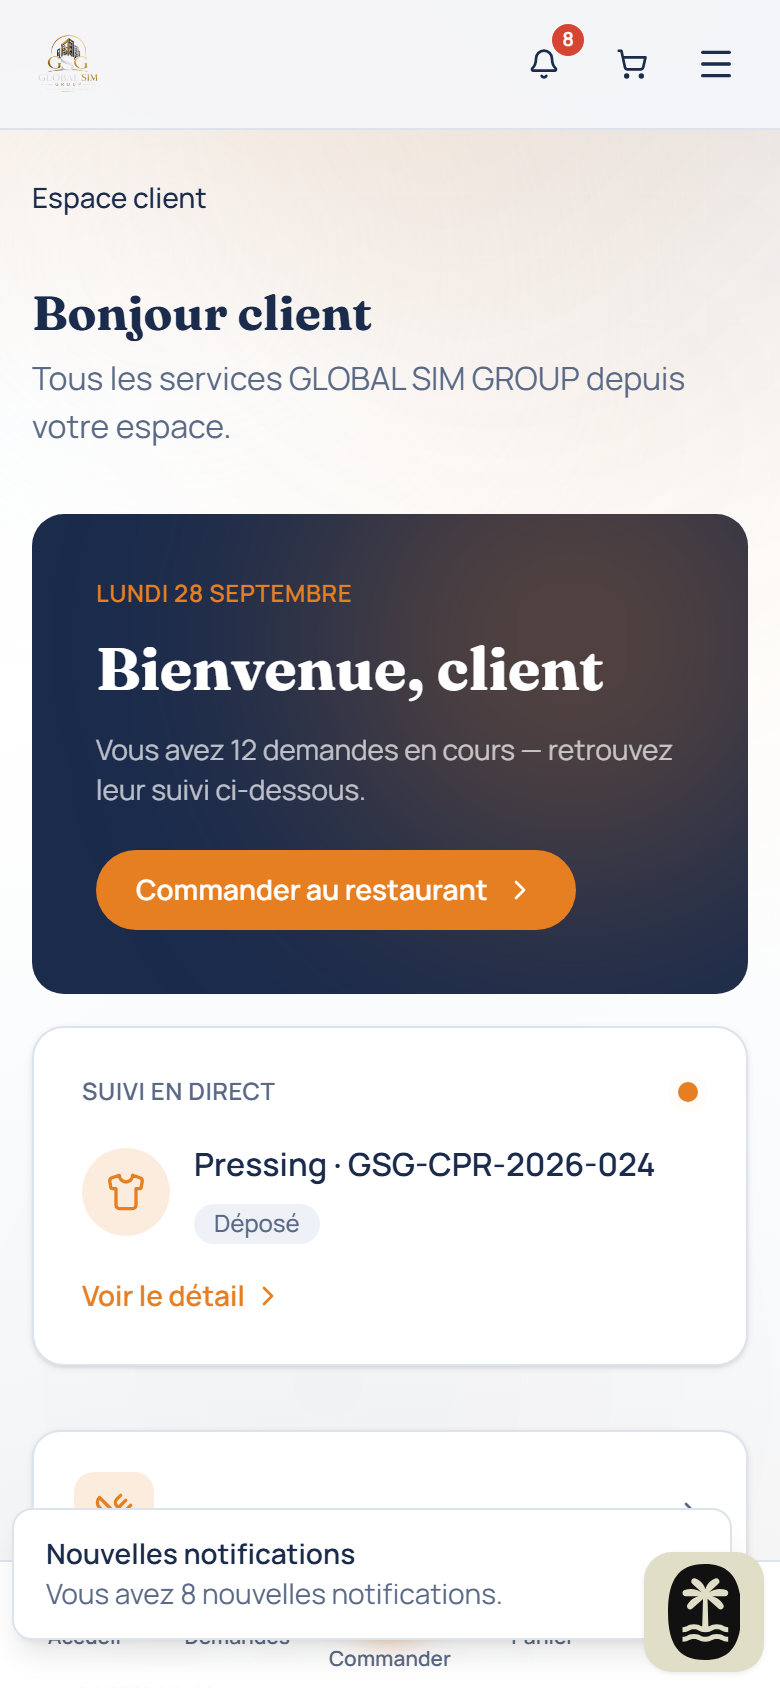
\includegraphics[width=\textwidth]{screenshots/espace-client/30-mobile-accueil.png}
  \captionof{figure}{L'accueil de l'espace client sur mobile}
\end{minipage}\hfill
\begin{minipage}{0.45\textwidth}
  \centering
  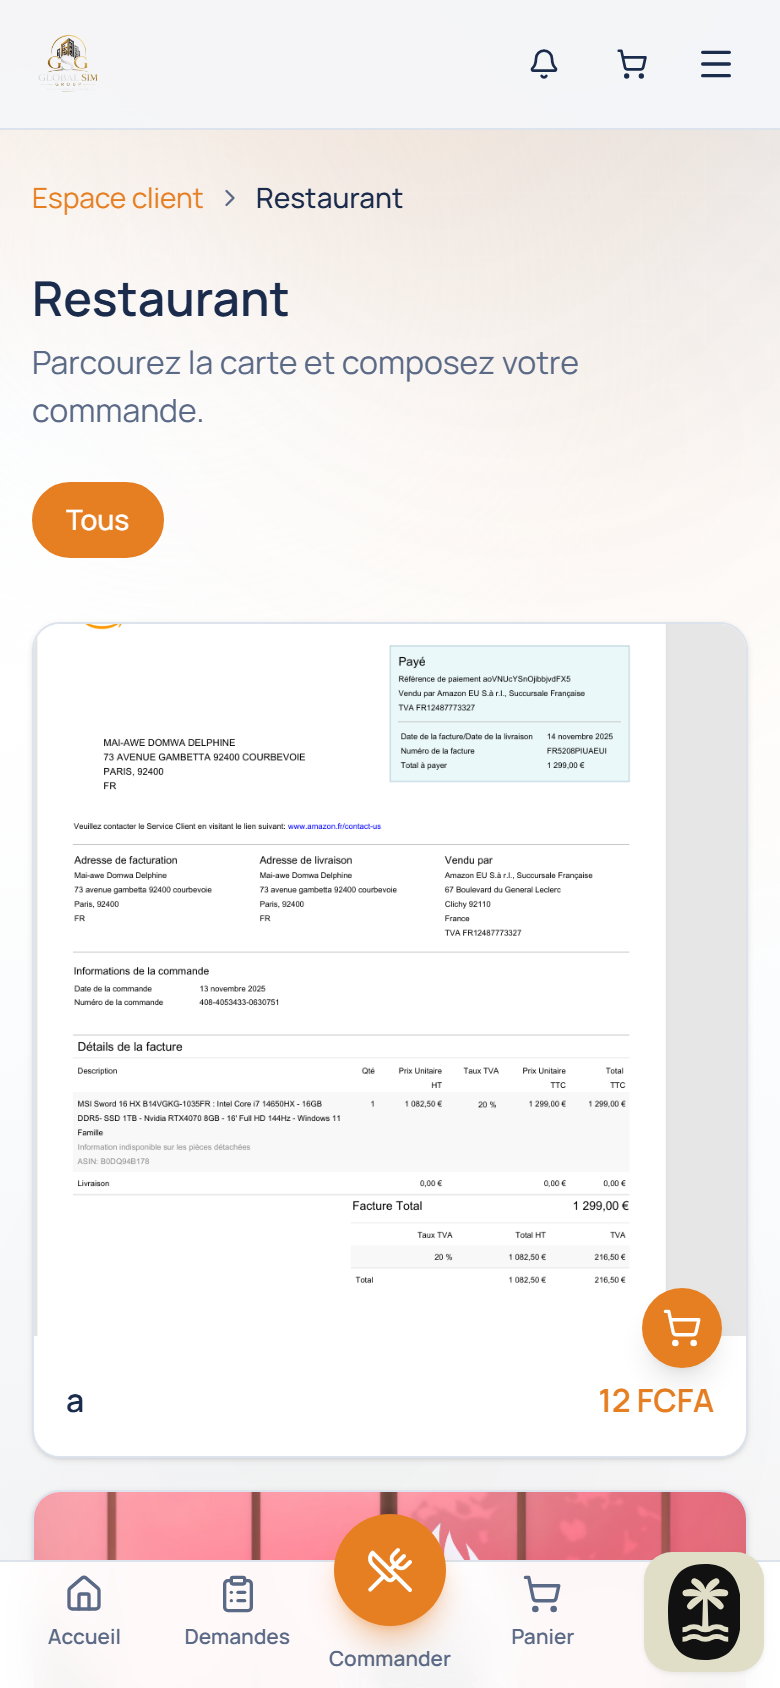
\includegraphics[width=\textwidth]{screenshots/espace-client/31-mobile-restaurant.png}
  \captionof{figure}{La carte du restaurant sur mobile}
\end{minipage}
\end{center}

\info{Même confort qu'à l'ordinateur : commandez un plat, demandez un produit ou signalez un problème depuis votre téléphone — les photos de l'appareil se joignent directement aux formulaires.}

\newpage

% FAQ
\section{J'ai un problème : que faire ?}

\begin{longtable}{>{\raggedright}p{5cm} p{9cm}}
\toprule
\textbf{Problème} & \textbf{Solution} \\
\midrule
\endfirsthead
\multicolumn{2}{c}{\textit{Suite de la FAQ}} \\
\toprule
\textbf{Problème} & \textbf{Solution} \\
\midrule
\endhead
\bottomrule
\endfoot

Je n'arrive pas à me connecter & Vérifiez l'identifiant et le mot de passe remis par la réception. En cas d'oubli, demandez à la réception de réinitialiser votre compte. \\

La page d'accueil ne s'ouvre pas & Il vous manque la permission \texttt{PORTAIL.VOIR} — demandez à la réception. \\

Je ne vois pas le bouton « Commander » / « Envoyer ma demande » & Chaque action demande sa permission (\texttt{RESTAURANT.COMMANDER}, \texttt{SALLE\_FETE.DEMANDER}…). Si le bouton manque, votre compte n'a pas le droit — demandez à la réception. \\

Mes articles ont disparu du panier & Le panier est stocké dans le navigateur : si vous videz le cache ou changez d'appareil, il repart à zéro. \\

La demande de séjour ne propose aucun logement & Il n'y a pas de logement libre sur ces dates, ou les deux dates ne sont pas encore remplies. Essayez une autre période. \\

Le formulaire de séjour refuse mes dates & L'arrivée doit être dans le futur et le départ après l'arrivée — corrigez les dates. \\

Un message dit que mon créneau « chevauche une réservation confirmée » & La salle est déjà prise sur cet horaire : décalez l'heure ou changez de date. L'encadré « Occupation du jour » montre les créneaux occupés. \\

Ma demande est restée « En attente de validation » & C'est normal : le personnel doit la traiter (disponibilité, tarif). Tant qu'elle est en attente, elle ne bloque ni le logement ni la salle — et vous pouvez l'annuler depuis sa fiche. \\

Comment annuler une demande ? & Ouvrez la fiche de la demande (restaurant, boutique, séjour, salle de fête, pressing) : le bouton \textbf{Annuler} est visible tant qu'elle n'a pas été validée par le personnel. \\

Le total de ma commande affiche « Total estimé » & Le montant est calculé sur les prix de la carte : le personnel peut l'ajuster à la validation (disponibilité, suppléments). Le montant définitif figure sur la fiche. \\

Je veux payer en ligne depuis l'espace client & Ce n'est pas prévu : tous les règlements se font sur place (réception, comptoir, caisse). L'espace sert à demander et à suivre. \\

Où sont mes échéances de loyer ? & Vous regardez l'espace client : le loyer, la caution et les états des lieux relèvent du \textbf{portail résident}, réservé aux comptes résidents. \\

\bottomrule
\end{longtable}

\newpage

\section{Récapitulatif des permissions}

Ce que votre compte client peut faire dépend de ses permissions — réglées par l'administration :

\begin{itemize}[label=\textcolor{lagoon}{\faKey}]
  \item \texttt{PORTAIL.VOIR} : ouvrir l'espace client et voir vos pages (catalogues, demandes, suivis).
  \item \texttt{RESTAURANT.COMMANDER} : passer une commande restaurant et l'annuler tant qu'elle est en attente.
  \item \texttt{MARCHANDISE.COMMANDER} : envoyer une demande d'achat boutique et l'annuler tant qu'elle est en attente.
  \item \texttt{RESIDENCE.DEMANDER} : envoyer une demande de séjour court et l'annuler tant qu'elle est en attente.
  \item \texttt{SALLE\_FETE.DEMANDER} : demander une réservation de salle de fête et l'annuler tant qu'elle est en attente.
  \item \texttt{PRESSING.DECLARER} : annuler une commande pressing encore en attente.
  \item \texttt{SIGNALEMENT.VOIR} : voir vos signalements.
  \item \texttt{SIGNALEMENT.CREER} : déclarer un signalement.
  \item \texttt{SIGNALEMENT.DECLARER\_TIERS} : déclarer un signalement pour le compte d'un tiers.
\end{itemize}

\info{Sans la permission, le bouton correspondant n'apparaît simplement pas : ce n'est pas un bug. Demandez à la réception de faire ajuster votre compte si un service vous manque.}

\vfill

\begin{center}
\begin{tikzpicture}
  \node[fill=sea-ink, text=white, rounded corners=10pt, minimum width=10cm, minimum height=1.5cm, font=\large\bfseries] {GLOBAL SIM GROUP, à votre service !};
\end{tikzpicture}
\end{center}

\end{document}
